%=============================================================================
%  VECM Multi-Step Forecasting -- Mathematical Notes & Documentation
%  vecm_forecast.py | Project Dark-Wing
%  Financial Mathematics / Time Series Analysis / Kalman_Filter
%=============================================================================
\documentclass[10pt,a4paper,twocolumn]{article}

%--- Geometry ----------------------------------------------------------------
\usepackage[a4paper,top=1.8cm,bottom=1.8cm,left=1.5cm,right=1.5cm,
            columnsep=0.7cm]{geometry}

%--- Math --------------------------------------------------------------------
\usepackage{amsmath,amssymb,amsthm,mathtools}

%--- Typography --------------------------------------------------------------
\usepackage[T1]{fontenc}
\usepackage{lmodern}
\usepackage{microtype}
\usepackage{parskip}
\setlength{\parskip}{2pt}

%--- Colours -----------------------------------------------------------------
\usepackage{xcolor}
\definecolor{codebg}{RGB}{245,247,250}
\definecolor{codeframe}{RGB}{180,195,220}
\definecolor{keyword}{RGB}{0,80,180}
\definecolor{comment}{RGB}{80,115,80}
\definecolor{string}{RGB}{160,40,20}
\definecolor{mathbluebg}{RGB}{230,240,255}
\definecolor{mathblue}{RGB}{10,60,160}
\definecolor{accent}{RGB}{25,95,195}
\definecolor{greenbg}{RGB}{230,250,232}
\definecolor{greenframe}{RGB}{50,155,70}
\definecolor{yellowbg}{RGB}{255,252,230}
\definecolor{yellowframe}{RGB}{180,150,0}
\definecolor{notebg}{RGB}{248,245,255}
\definecolor{noteframe}{RGB}{120,80,180}

%--- Code listings -----------------------------------------------------------
\usepackage{listings}
\lstdefinestyle{pythonplain}{
  language=Python,
  backgroundcolor=\color{codebg},
  frame=single,rulecolor=\color{codeframe},
  basicstyle=\ttfamily\fontsize{6.5}{8}\selectfont,
  keywordstyle=\bfseries\color{keyword},
  commentstyle=\itshape\color{comment},
  stringstyle=\color{string},
  numbers=none,breaklines=true,tabsize=2,
  showstringspaces=false,aboveskip=3pt,belowskip=3pt,
  xleftmargin=4pt,
}

%--- TikZ --------------------------------------------------------------------
\usepackage{tikz}
\usetikzlibrary{shapes.geometric,arrows.meta,positioning,calc,
                backgrounds,decorations.pathreplacing,fit}
\raggedbottom

\tikzset{
  fc_start/.style={rectangle,rounded corners=5pt,
    draw=accent,fill=accent!18,
    text width=4.4cm,align=center,
    font=\footnotesize\bfseries,
    inner sep=4pt,minimum height=0.6cm},
  fc_proc/.style={rectangle,
    draw=black!55,fill=white,
    text width=4.4cm,align=center,
    font=\footnotesize,
    inner sep=3pt,minimum height=0.58cm},
  fc_dec/.style={diamond,aspect=2.5,
    draw=accent,fill=accent!9,
    text width=2.9cm,align=center,
    font=\fontsize{6.2}{7.2}\selectfont,
    inner sep=1pt},
  fc_out/.style={rectangle,rounded corners=3pt,
    draw=greenframe,fill=greenbg,
    text width=4.4cm,align=center,
    font=\footnotesize,
    inner sep=3pt,minimum height=0.58cm},
  fc_side/.style={rectangle,
    draw=black!45,fill=yellow!10,
    text width=2.0cm,align=center,
    font=\fontsize{6.2}{7.2}\selectfont,
    inner sep=2pt,minimum height=0.52cm},
  arr/.style={-Stealth,semithick,draw=black!65},
}

%--- Boxes -------------------------------------------------------------------
\usepackage[most]{tcolorbox}
\tcbset{
  mathbox/.style={colback=mathbluebg,colframe=mathblue,
    fonttitle=\bfseries\small,title=#1,
    boxrule=0.5pt,top=3pt,bottom=3pt,left=4pt,right=4pt,
    before skip=4pt,after skip=4pt},
  exbox/.style={colback=yellowbg,colframe=yellowframe,
    fonttitle=\bfseries\small,title=#1,
    boxrule=0.5pt,top=3pt,bottom=3pt,left=4pt,right=4pt,
    before skip=4pt,after skip=4pt},
  resultbox/.style={colback=greenbg,colframe=greenframe,
    fonttitle=\bfseries\small,title=#1,
    boxrule=0.5pt,top=3pt,bottom=3pt,left=4pt,right=4pt,
    before skip=4pt,after skip=4pt},
  codebox/.style={colback=codebg,colframe=codeframe,
    fonttitle=\bfseries\small\color{accent},title=#1,
    boxrule=0.5pt,top=2pt,bottom=2pt,left=2pt,right=2pt,
    before skip=4pt,after skip=4pt},
  notebox/.style={colback=notebg,colframe=noteframe,
    fonttitle=\bfseries\small,title=#1,
    boxrule=0.5pt,top=3pt,bottom=3pt,left=4pt,right=4pt,
    before skip=4pt,after skip=4pt},
}

%--- Tables ------------------------------------------------------------------
\usepackage{booktabs,array,multirow,colortbl}

%--- Header / Footer ---------------------------------------------------------
\usepackage{fancyhdr}
\usepackage[hidelinks]{hyperref}
\pagestyle{fancy}\fancyhf{}
\fancyhead[L]{\footnotesize\textbf{VECM Forecasting --- Study Notes}}
\fancyhead[R]{\footnotesize Project Dark-Wing}
\fancyfoot[C]{\footnotesize\thepage}
\renewcommand{\headrulewidth}{0.4pt}

%--- Floats / Captions -------------------------------------------------------
\usepackage{float,caption,graphicx}
\captionsetup{font=scriptsize,labelfont=bf,skip=3pt}

%--- Section formatting ------------------------------------------------------
\usepackage{titlesec}
\titlespacing*{\section}{0pt}{7pt}{3pt}
\titlespacing*{\subsection}{0pt}{5pt}{2pt}
\titlespacing*{\subsubsection}{0pt}{3pt}{1pt}
\titleformat{\section}{\normalfont\bfseries\color{accent}}{}{0em}{}
  [{\color{accent}\titlerule[0.5pt]}]
\titleformat{\subsection}{\normalfont\bfseries\small}{}{0em}{}
\titleformat{\subsubsection}{\normalfont\itshape\small}{}{0em}{}

%--- Macros ------------------------------------------------------------------
\newcommand{\Delt}{\Delta}
\newcommand{\bPi}{\boldsymbol{\Pi}}
\newcommand{\balpha}{\boldsymbol{\alpha}}
\newcommand{\bbeta}{\boldsymbol{\beta}}
\newcommand{\bGamma}{\boldsymbol{\Gamma}}
\newcommand{\bSigma}{\boldsymbol{\Sigma}}
\newcommand{\bPhi}{\boldsymbol{\Phi}}
\newcommand{\beps}{\boldsymbol{\varepsilon}}
\newcommand{\rstar}{r^{*}}

\begin{document}

\twocolumn[{%
\begin{center}
  {\LARGE\bfseries\color{accent} Vector Error Correction Model (VECM) Forecasting}\\[5pt]
  {\large\bfseries \texttt{vecm\_forecast.py} --- Mathematical Notes \& Documentation}\\[3pt]
  {\small\itshape Companion VAR Level Projection, Cointegrated Spread Estimation, \& Growing MSE Bands}\\[3pt]
  {\small Project Dark-Wing \quad|\quad \today}
\end{center}
\vspace{4pt}
\noindent\rule{\linewidth}{0.5pt}\vspace{2pt}
\begin{quote}\small
\textbf{Abstract.}~While structural VECM describes the short-run differenced dynamics and long-run equilibrium cointegration constraints of non-stationary $I(1)$ assets, multi-step-ahead forecasting requires projecting the actual \emph{price levels} into the future. This is accomplished by mapping the fitted VECM parameters into its companion Vector Autoregressive (VAR) levels representation. From these forecasted levels, we project the cointegrated portfolio spread (Error Correction Term) and compute its analytical forecast Mean Squared Error (MSE) matrix to derive dynamic confidence bands. This document outlines the levels representation conversion, derives the analytical MSE propagation, provides a step-by-step numerical worked example, and details the implementation in \texttt{vecm\_forecast.py}.
\end{quote}
\noindent\rule{\linewidth}{0.5pt}\vspace{5pt}
}]

%=============================================================================
\section{Motivation: Levels vs.\ Differences}
%=============================================================================

In Granger's Representation Theorem, a cointegrated system of assets $X_t \in \mathbb{R}^m$ is represented in differences $\Delt X_t = X_t - X_{t-1}$ to maintain stationarity, while modeling the long-run relations via levels:
\[
  \Delt X_t = \balpha \bbeta' X_{t-1} + \sum_{i=1}^{k-1} \bGamma_i \Delt X_{t-i} + \beps_t
\]
where $\bbeta'$ is the $(r^* \times m)$ cointegrating matrix mapping the $I(1)$ levels to $r^*$ stationary portfolios (spreads), and $\balpha$ is the $(m \times r^*)$ speed of adjustment matrix.

For a pairs trader, forecasting the differenced series $\Delt X_{T+h}$ is of limited direct use. We require:
\begin{enumerate}\setlength\itemsep{0pt}
  \item The forecast of the asset \emph{price levels} $X_{T+h}$ to evaluate capital constraints and contract sizes.
  \item The forecast of the \emph{spread level} $S_{T+h} = \bbeta' X_{T+h}$ to verify if the spread is expected to mean-revert to zero, indicating entry feasibility and target hold times.
\end{enumerate}

Thus, we must transform the VECM into a Vector Autoregression (VAR) in levels, compute the level forecasts recursively, and project the spread.

%=============================================================================
\section{The Companion VAR Levels Form}
%=============================================================================

A Vector Autoregression of order $k$ (in levels) is written as:
\begin{equation}
  X_t = A_1 X_{t-1} + A_2 X_{t-2} + \dots + A_k X_{t-k} + \beps_t
  \label{eq:var_levels}
\end{equation}

To convert a VECM with $k-1$ lag differences into this VAR(k) levels form, we expand the differences $\Delt X_{t-i} = X_{t-i} - X_{t-i-1}$ and collect terms at identical lags.

\begin{tcolorbox}[mathbox={VECM to VAR Levels Transformation}]
Let the VECM model be:
\[
  X_t - X_{t-1} = \bPi X_{t-1} + \bGamma_1 (X_{t-1} - X_{t-2}) + \dots + \bGamma_{k-1} (X_{t-k+1} - X_{t-k}) + \beps_t
\]
where $\bPi = \balpha \bbeta'$. Collecting the level coefficients $A_j$ for Eq.~\eqref{eq:var_levels}:
\begin{align}
  A_1 &= I_m + \bPi + \bGamma_1 \label{eq:a1} \\
  A_j &= \bGamma_j - \bGamma_{j-1} \quad \text{for } 2 \le j \le k-1 \label{eq:aj} \\
  A_k &= -\bGamma_{k-1} \label{eq:ak}
\end{align}
\end{tcolorbox}

\subsection{Proof of the Conversion}
Let us write down the VECM equation explicitly:
\[
  X_t = X_{t-1} + \bPi X_{t-1} + \bGamma_1 X_{t-1} - \bGamma_1 X_{t-2} + \dots + \bGamma_{k-1} X_{t-k+1} - \bGamma_{k-1} X_{t-k} + \beps_t
\]
Grouping the terms by the lag of $X$:
\begin{itemize}
  \item For $X_{t-1}$: Coefficient is $I_m + \bPi + \bGamma_1$. This matches Eq.~\eqref{eq:a1}.
  \item For $X_{t-j}$ (where $2 \le j \le k-1$): The term $X_{t-j}$ appears in the expansion of $\bGamma_j \Delt X_{t-j}$ as $\bGamma_j X_{t-j}$ and in $\bGamma_{j-1} \Delt X_{t-j+1}$ as $-\bGamma_{j-1} X_{t-j}$. Thus, the collected coefficient is $\bGamma_j - \bGamma_{j-1}$. This matches Eq.~\eqref{eq:aj}.
  \item For $X_{t-k}$: The only term containing $X_{t-k}$ is the negative part of the last difference: $-\bGamma_{k-1} X_{t-k}$. Thus, the coefficient is $-\bGamma_{k-1}$. This matches Eq.~\eqref{eq:ak}.
\end{itemize}
This completes the derivation. The representation is identical and preserves the long-run cointegration properties of the VECM system.

%=============================================================================
\section{Multi-step-ahead Level Recursion}
%=============================================================================

For forecasting from time $T$, we take the conditional expectation relative to the filtration $\mathcal{F}_T$. Let $\hat{X}_{T+h|T} = \mathbb{E}[X_{T+h} \mid \mathcal{F}_T]$.

\begin{tcolorbox}[mathbox={VAR levels h-Step Recursion}]
For $h = 1, 2, \dots, H$:
\begin{equation}
  \hat{X}_{T+h|T} = \sum_{j=1}^{k} A_j \hat{X}_{T+h-j|T}
  \label{eq:levels_rec}
\end{equation}
where:
\[
  \hat{X}_{T+h-j|T} = X_{T+h-j} \quad \text{if } h-j \le 0 \quad \text{(historical data)}
\]
and the deterministic components (constants/trends) are added according to the chosen VECM specification.
\end{tcolorbox}

%=============================================================================
\section{Spread (ECT) Forecasting}
%=============================================================================

Once the level forecasts $\hat{X}_{T+h|T}$ are obtained, the cointegrated spread portfolio (Error Correction Term) forecast vector $\hat{S}_{T+h|T} \in \mathbb{R}^{r^*}$ is directly projected:

\begin{tcolorbox}[mathbox={ECT Portfolio Forecast}]
\begin{equation}\label{eq:ect_fc}
  \hat{S}_{T+h|T} = \bbeta' \hat{X}_{T+h|T}
\end{equation}
Because the levels $X_t$ are tied by the cointegrating vector $\bbeta$, the levels forecast $\hat{X}_{T+h|T}$ guarantees that $\hat{S}_{T+h|T}$ converges dynamically to the long-run mean of the cointegrated relation.
\end{tcolorbox}

%=============================================================================
\section{Forecast Error and MSE Propagation}
%=============================================================================

\subsection{MA Representation of levels VAR}
To compute the forecast error variance of the levels and the spread, we express the VAR(k) system in its Vector Moving Average, $\text{VMA}(\infty)$, form:
\[
  X_t = \sum_{j=0}^{\infty} \bPhi_j \beps_{t-j}
\]
where the coefficient matrices $\bPhi_j$ are calculated recursively using the autoregressive matrices $A_i$:
\begin{equation}
  \bPhi_0 = I_m, \quad \bPhi_j = \sum_{i=1}^{\min(j, k)} A_i \bPhi_{j-i} \quad \text{for } j \ge 1
  \label{eq:ma_coef}
\end{equation}

\subsection{Price Level MSE}
The forecast error at horizon $h$ is:
\[
  e_{T}(h) = X_{T+h} - \hat{X}_{T+h|T} = \sum_{j=0}^{h-1} \bPhi_j \beps_{T+h-j}
\]
Assuming $\beps_t$ is white noise with covariance matrix $\bSigma_u$, the Mean Squared Error (MSE) matrix of the price levels forecast is:
\begin{tcolorbox}[mathbox={Levels Forecast MSE Matrix}]
\begin{equation}
  \bSigma_X(h) = \text{Var}(e_{T}(h)) = \sum_{j=0}^{h-1} \bPhi_j \bSigma_u \bPhi_j'
  \label{eq:levels_mse}
\end{equation}
The diagonal elements of $\bSigma_X(h)$ represent the forecast variance of each individual asset level at horizon $h$.
\end{tcolorbox}

\subsection{Spread Forecast MSE}
The forecast error of the cointegrated spread portfolio is:
\[
  e_S(h) = S_{T+h} - \hat{S}_{T+h|T} = \bbeta' \left( X_{T+h} - \hat{X}_{T+h|T} \right) = \bbeta' e_T(h)
\]

\begin{tcolorbox}[mathbox={Spread Forecast Variance and Confidence Bands}]
The variance matrix of the forecasted spread $\hat{S}_{T+h|T}$ is:
\begin{equation}
  \bSigma_S(h) = \bbeta' \bSigma_X(h) \bbeta = \sum_{j=0}^{h-1} \left( \bbeta' \bPhi_j \right) \bSigma_u \left( \bbeta' \bPhi_j \right)'
  \label{eq:spread_mse}
\end{equation}
The standard error for the $i$-th spread portfolio is:
\[
  \text{SE}_i(h) = \sqrt{[\bSigma_S(h)]_{ii}}
\]
The corresponding $(1-\alpha)$ confidence bands are:
\begin{equation}
  \text{CI}_i(h) = [\hat{S}_{T+h|T}]_i \pm z_{\alpha/2} \, \text{SE}_i(h)
\end{equation}
\end{tcolorbox}

%=============================================================================
\section{Reversion Horizon $h^*$}
%=============================================================================

In statistical arbitrage, we enter a trade when the spread deviates from its mean. The VECM forecast helps us estimate how many periods it will take for the spread to cross the equilibrium line (zero, for a de-meaned spread).

\begin{tcolorbox}[mathbox={Zero-Crossing Horizon $h^*$}]
For a given spread index $i$:
\begin{equation}
  h^* = \min \left\{ h \in \{1, \dots, H\} \mid \text{sign}( [\hat{S}_{T+h|T}]_i ) \neq \text{sign}( [\hat{S}_{T|T}]_i ) \right\}
\end{equation}
If no sign change occurs within $H$, $h^*$ is undefined (spread does not cross zero in the forecast window).
\end{tcolorbox}

%=============================================================================
\section{Worked Numerical Example}
%=============================================================================

\begin{tcolorbox}[exbox={2-Asset Cointegrated System Setup}]
Let $m=2$, $k=1$ (VAR order). The VECM has no lag differences:
\[
  \Delt X_t = \balpha \bbeta' X_{t-1} + \beps_t
\]
Let:
\[
  \balpha = \begin{bmatrix} -0.2 \\ 0.1 \end{bmatrix}, \quad
  \bbeta = \begin{bmatrix} 1.0 \\ -2.0 \end{bmatrix}, \quad
  \bSigma_u = \begin{bmatrix} 0.01 & 0.00 \\ 0.00 & 0.02 \end{bmatrix}
\]
Hence:
\[
  \bPi = \balpha \bbeta' = \begin{bmatrix} -0.2(1) & -0.2(-2) \\ 0.1(1) & 0.1(-2) \end{bmatrix} = \begin{bmatrix} -0.2 & 0.4 \\ 0.1 & -0.2 \end{bmatrix}
\]
The initial state at $T$ is $X_T = [10.0, 4.8]'$ and current spread is:
\[
  S_T = \bbeta' X_T = 1.0(10.0) - 2.0(4.8) = 0.4
\]
\end{tcolorbox}

\subsubsection{Step 1: Convert to VAR Levels Matrix}
Since $k=1$, Eq.~\eqref{eq:a1} gives:
\[
  A_1 = I_2 + \bPi = \begin{bmatrix} 1 & 0 \\ 0 & 1 \end{bmatrix} + \begin{bmatrix} -0.2 & 0.4 \\ 0.1 & -0.2 \end{bmatrix} = \begin{bmatrix} 0.8 & 0.4 \\ 0.1 & 0.8 \end{bmatrix}
\]

\subsubsection{Step 2: Level Forecasts}
For $h=1$:
\[
  \hat{X}_{T+1|T} = A_1 X_T = \begin{bmatrix} 0.8 & 0.4 \\ 0.1 & 0.8 \end{bmatrix} \begin{bmatrix} 10.0 \\ 4.8 \end{bmatrix} = \begin{bmatrix} 9.92 \\ 4.84 \end{bmatrix}
\]
For $h=2$:
\[
  \hat{X}_{T+2|T} = A_1 \hat{X}_{T+1|T} = \begin{bmatrix} 0.8 & 0.4 \\ 0.1 & 0.8 \end{bmatrix} \begin{bmatrix} 9.92 \\ 4.84 \end{bmatrix} = \begin{bmatrix} 9.872 \\ 4.864 \end{bmatrix}
\]

\subsubsection{Step 3: Spread Forecasts}
For $h=1$:
\[
  \hat{S}_{T+1|T} = \bbeta' \hat{X}_{T+1|T} = 1.0(9.92) - 2.0(4.84) = 0.24
\]
For $h=2$:
\[
  \hat{S}_{T+2|T} = \bbeta' \hat{X}_{T+2|T} = 1.0(9.872) - 2.0(4.864) = 0.144
\]
Note the spread is mean-reverting (0.40 $\to$ 0.24 $\to$ 0.144).

\subsubsection{Step 4: MA Coefficients and MSE}
Using Eq.~\eqref{eq:ma_coef}:
\[
  \bPhi_0 = I_2, \quad \bPhi_1 = A_1 = \begin{bmatrix} 0.8 & 0.4 \\ 0.1 & 0.8 \end{bmatrix}
\]
For $h=1$, levels MSE:
\[
  \bSigma_X(1) = \bPhi_0 \bSigma_u \bPhi_0' = \bSigma_u = \begin{bmatrix} 0.01 & 0.00 \\ 0.00 & 0.02 \end{bmatrix}
\]
Spread variance at $h=1$:
\begin{align*}
  \bSigma_S(1) &= \bbeta' \bSigma_X(1) \bbeta = \begin{bmatrix} 1 & -2 \end{bmatrix} \begin{bmatrix} 0.01 & 0.00 \\ 0.00 & 0.02 \end{bmatrix} \begin{bmatrix} 1 \\ -2 \end{bmatrix} \\
               &= 0.01 + (-2)^2(0.02) = 0.01 + 0.08 = 0.09
\end{align*}
Hence standard error at $h=1$: $\text{SE}(1) = \sqrt{0.09} = 0.3$.
The 95\% confidence interval of the spread at $h=1$ is:
\[
  \text{CI}(1) = 0.24 \pm 1.96(0.3) = 0.24 \pm 0.588 = [-0.348, 0.828]
\]

%=============================================================================
\section{Class Structure \& Flowchart}
%=============================================================================

\begin{figure}[H]
\centering
\resizebox{\columnwidth}{!}{%
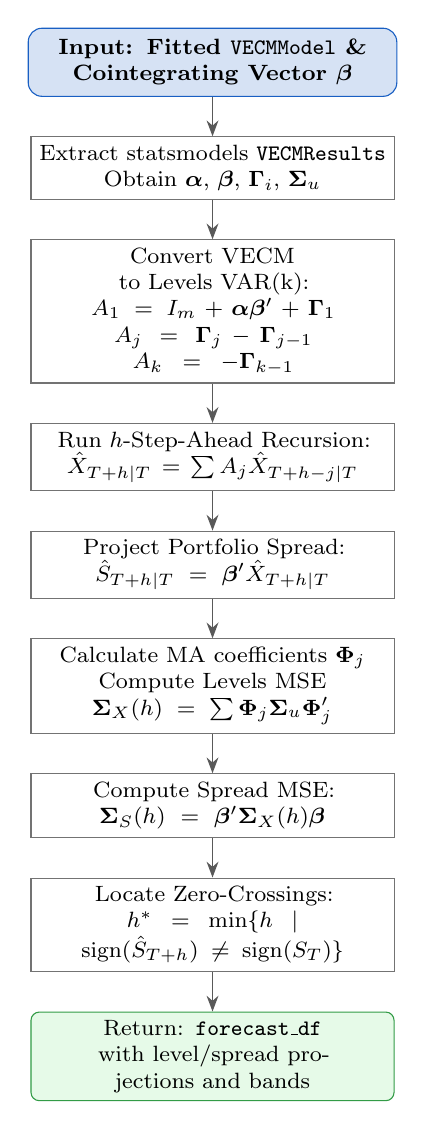
\begin{tikzpicture}[node distance=0.5cm,every node/.style={font=\scriptsize}]
  \node (in) [fc_start] {Input: Fitted \texttt{VECMModel} \& Cointegrating Vector $\bbeta$};
  \node (init) [fc_proc,below=of in] {Extract statsmodels \texttt{VECMResults}\\ Obtain $\balpha$, $\bbeta$, $\bGamma_i$, $\bSigma_u$};
  \node (conv) [fc_proc,below=of init] {Convert VECM to Levels VAR(k):\\
    $A_1 = I_m + \balpha\bbeta' + \bGamma_1$\\
    $A_j = \bGamma_j - \bGamma_{j-1}$\\
    $A_k = -\bGamma_{k-1}$};
  \node (rec) [fc_proc,below=of conv] {Run $h$-Step-Ahead Recursion:\\
    $\hat{X}_{T+h|T} = \sum A_j \hat{X}_{T+h-j|T}$};
  \node (proj) [fc_proc,below=of rec] {Project Portfolio Spread:\\
    $\hat{S}_{T+h|T} = \bbeta' \hat{X}_{T+h|T}$};
  \node (ma) [fc_proc,below=of proj] {Calculate MA coefficients $\bPhi_j$\\
    Compute Levels MSE $\bSigma_X(h) = \sum \bPhi_j \bSigma_u \bPhi_j'$};
  \node (var) [fc_proc,below=of ma] {Compute Spread MSE:\\
    $\bSigma_S(h) = \bbeta' \bSigma_X(h) \bbeta$};
  \node (cross) [fc_proc,below=of var] {Locate Zero-Crossings:\\
    $h^* = \min \{h \mid \text{sign}(\hat{S}_{T+h}) \neq \text{sign}(S_T)\}$};
  \node (out) [fc_out,below=of cross] {Return: \texttt{forecast\_df}\\
    with level/spread projections and bands};
  \draw[arr] (in) -- (init);
  \draw[arr] (init) -- (conv);
  \draw[arr] (conv) -- (rec);
  \draw[arr] (rec) -- (proj);
  \draw[arr] (proj) -- (ma);
  \draw[arr] (ma) -- (var);
  \draw[arr] (var) -- (cross);
  \draw[arr] (cross) -- (out);
\end{tikzpicture}
}
\caption{System flowchart of the \texttt{VECMForecaster} class.}
\end{figure}

%=============================================================================
\section{Python Implementation Snippets}
%=============================================================================

\begin{tcolorbox}[codebox={\texttt{vecm\_forecast.py} Main Methods}]
\begin{lstlisting}[style=pythonplain]
class VECMForecaster:
    def __init__(self, vecm_model, alpha_level=0.05):
        self._vm = vecm_model
        self._result = vecm_model._fitted_result
        self._beta = vecm_model.get_beta() # (m x r*)
        self._alpha_conf = alpha_level
        self._z_crit = float(stats.norm.ppf(1 - alpha_level/2))
        
    def forecast(self, steps=20):
        self._steps = steps
        # statsmodels handles conversion internally for level prediction
        fc_array = self._result.predict(steps=steps)
        cols = self._result.model.endog_names
        # ... generate DatetimeIndex ...
        self._price_fc = pd.DataFrame(fc_array[:steps], index=future_idx, columns=cols)
        return self._price_fc

    def spread_forecast(self, steps=None):
        if steps is not None:
            self.forecast(steps)
        fc_values = self._price_fc.values # (steps x m)
        beta = self._beta # (m x r*)
        spread_fc = fc_values @ beta # (steps x r*)
        self._spread_fc = pd.DataFrame(spread_fc, index=self._price_fc.index,
                                       columns=[f"ECT_{j+1}" for j in range(beta.shape[1])])
        return self._spread_fc
\end{lstlisting}
\tcblower
\begin{lstlisting}[style=pythonplain]
    def confidence_bands(self, steps=None, alpha=None):
        if steps is not None:
            self.forecast(steps)
        if self._spread_fc is None:
            self.spread_forecast()
        h = len(self._price_fc)
        ma_coef = self._result.ma_rep(maxn=h) # (h x m x m)
        sigma_u = self._result.sigma_u # (m x m)
        
        m = sigma_u.shape[0]
        mse = np.zeros((h, m, m))
        cumulative = np.zeros((m, m))
        for step in range(h):
            Phi = ma_coef[step]
            cumulative += Phi @ sigma_u @ Phi.T
            mse[step] = cumulative.copy()
            
        beta = self._beta # (m x r*)
        r = beta.shape[1]
        spread_se = np.zeros((h, r))
        for step in range(h):
            var_mat = beta.T @ mse[step] @ beta
            spread_se[step] = np.sqrt(np.maximum(np.diag(var_mat), 0))
            
        se_df = pd.DataFrame(spread_se, index=self._spread_fc.index, columns=self._spread_fc.columns)
        upper = self._spread_fc + self._z_crit * se_df
        lower = self._spread_fc - self._z_crit * se_df
        return {"upper": upper, "lower": lower, "se": se_df, "point": self._spread_fc}
\end{lstlisting}
\end{tcolorbox}

%=============================================================================
\section{Interview Preparation}
%=============================================================================

\begin{tcolorbox}[exbox={Key VECM Forecasting Questions}]
\begin{enumerate}\setlength\itemsep{1pt}
  \item \textbf{Why can't we forecast a VECM by simply forecasting the differences and integrating?}\\
    Doing so is possible but mathematically cumbersome for keeping track of the levels covariance. Converting to the companion VAR levels form provides a unified statespace layout for computing exact levels covariance at any horizon.
  \item \textbf{What is the long-run behavior of $\hat{S}_{T+h|T}$?}\\
    Since $S_t = \bbeta' X_t$ is stationary, the forecast $\hat{S}_{T+h|T}$ must converge to the unconditional mean (constant term in the cointegration relation) as $h \to \infty$. If de-meaned, it converges to zero.
  \item \textbf{Why do the confidence bands of the spread stabilize while those of the levels grow to infinity?}\\
    The level prices $X_t$ are $I(1)$ (unit roots), so their forecast variance grows without bound ($\bSigma_X(h) \to \infty$ as $h \to \infty$). However, the spread is $I(0)$, so its variance $\bbeta'\bSigma_X(h)\bbeta$ converges to the stationary variance of the spread portfolio.
  \item \textbf{How does VECM forecast help in setting trade exit points?}\\
    The zero-crossing horizon $h^*$ represents the statistical expectation of the trade duration. If $h^*$ is longer than the assets' options expiry or your capital cost horizon, the trade may be rejected.
\end{enumerate}
\end{tcolorbox}

%=============================================================================
\section{Pipeline Position}
%=============================================================================

\begin{center}{\small
\begin{tabular}{@{}clp{2.5cm}@{}}
\toprule Step & Module & Output\\\midrule
4 & \texttt{fit\_vecm.py} & Cointegrating relations\\
4.5 & \texttt{diagnostics.py} & Residual validation\\
5 & \texttt{spread\_builder.py} & OLS / ECT spread\\
6 & \texttt{kalman\_filter.py} & Filtering states\\
\textbf{7a} & \textbf{\texttt{vecm\_forecast.py}} & Levels / Spread forecast\\
7b & \texttt{kalman\_forecast.py} & State projection\\
8 & \texttt{signal/pair\_signal.py} & Trading entries\\
\bottomrule
\end{tabular}
}\end{center}

\end{document}